%! Author = maad
%! Date = 01.08.2024

\chapter{Perceptron}\label{ch:perceptron}

The following books explain the contents of this chapter in more detail: \textit{Haykin, 2009}~\cite{HaykinNeural2009};
\textit{Goodfellow, 2016}~\cite{GoodfellowDeep2016}; \textit{Bishop, 2006}~\cite{BishopPattern2006};
\textit{Calin, 2020}~\cite{CalinDeep2020}; \textit{Aggarwal, 2018}~\cite{AggarwalNeural2018}.

Perceptron potential, where $I_b$ is the number of inputs and $b$ is the bias:

\begin{equation}\label{eq:perceptron-potential}
    v = \sum_{i=1}^{I_b} w_i x_i + b
\end{equation}

The bias can be embedded into the input vector:

\begin{equation}\label{eq:m-plus-one-0}
    I = I_b + 1
\end{equation}

\begin{equation}\label{eq:perceptron-potential-2}
    \bm{x} =
    \begin{bmatrix}
        x_1 & x_2 & \ldots & x_{I_b} & 1
    \end{bmatrix}^T \ , \quad
    \bm{w} =
    \begin{bmatrix}
        w_1 & w_2 & \ldots & w_{I_b} & b
    \end{bmatrix}^T
\end{equation}

\begin{equation}\label{eq:perceptron-potential-3}
v = \sum_{i=1}^{I} w_i x_i
\end{equation}

Perceptron output:

\begin{equation}\label{eq:perceptron-output}
    y = \phi (v)
\end{equation}


\subsection{Output in vector form}\label{subsec:vector-form}

The bias $b$ has been embedded into the vectors $\bm{x}$ and $\bm{w}$:

\begin{equation}\label{eq:perceptron-vector}
y = \phi (\bm{w}^T \bm{x})
\end{equation}


\section{Activation functions and their derivatives}\label{sec:activation-functions}


\subsection{Sigmoid}\label{subsec:sigmoid}

\begin{equation}\label{eq:activation-sigmoid}
    \phi (v) = \frac{1}{1 + \exp(- v)}
\end{equation}

\begin{equation}\label{eq:activation-sigmoid-derivative}
    \phi' (v) = \phi (v) (1 - \phi (v))
\end{equation}


\subsection{Hyperbolic tangent}\label{subsec:hyperbolic-tangent}

\begin{equation}\label{eq:activation-tanh}
    \phi (v) = \tanh (v)
\end{equation}

\begin{equation}\label{eq:activation-tanh-derivative}
    \phi' (v) = 1 - \phi (v)^2
\end{equation}


\subsection{Rectified linear unit (ReLU)}\label{subsec:relu}

\begin{equation}\label{eq:activation-relu}
    \phi (v) = \max (0, v)
\end{equation}

\begin{equation}\label{eq:activation-relu-derivative}
    \phi' (v) =
    \begin{cases}
        0 & \text{if } v < 0 \\
        1 & \text{if } v > 0
    \end{cases}
\end{equation}

\section{Figures}\label{sec:figures-perceptron}

\begin{figure}[H]
    \centering
    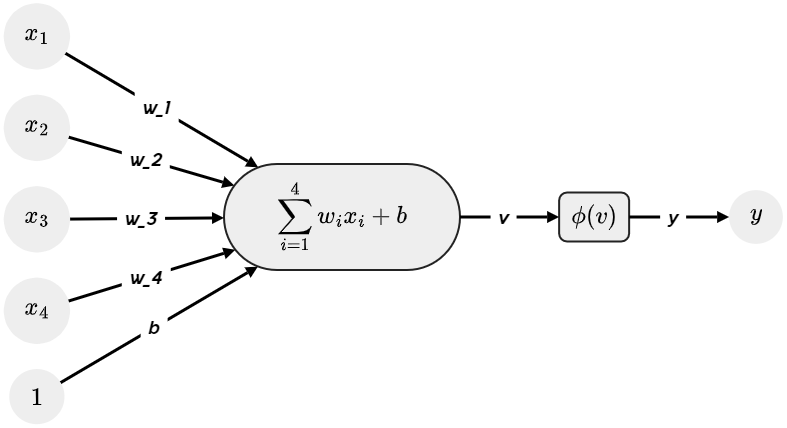
\includegraphics[width=0.8\textwidth]{figures/perceptron/Perceptron1c}
    \caption[Caption used in list of tables]{The basic structure of a perceptron~\cite{MaadCookbook2024}.}
    \label{fig:Perceptron1}
\end{figure}

